\section{Mais quelle est donc cette matière ? (4 points)}

Nolan ne se rappelle plus quel plastique il doit acheter pour son imprimante 3D : de l'ABS ou du PLA ?

\begin{itemize}
	\item \textbf{L'ABS} est un plastique courant, on le retrouve dans les Lego par exemple. Son point fort vient de sa solidité, il commence à fondre à 180°C.
	
	\item Issu de matériaux recyclés, tels que l'amidon de maïs \textbf{le PLA} est une matière plus naturelle et biodégradable. Sa température de fusion est de 160°C.	
\end{itemize}

\begin{questions}
	\question[2] Quelle expérience Nolan peut-il réaliser pour identifier le plastique de son imprimante ?
<<<<<<< HEAD
	
	\question[2] Il trace l'évolution de la température pendant la fusion du plastique. Quel est le plastique de son imprimante ?
	
	\begin{center}
		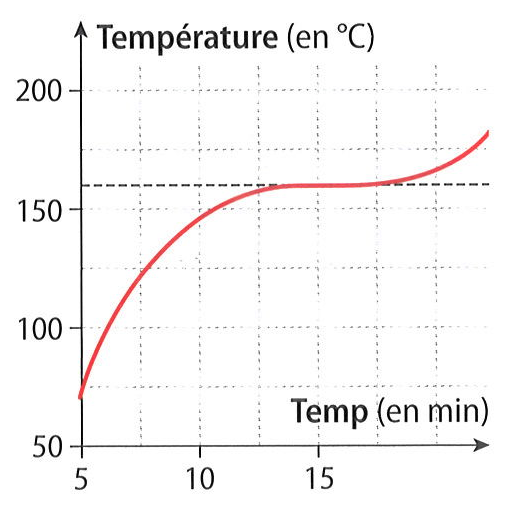
\includegraphics[scale=0.6]{img/courbe2}
	\end{center}
=======
		\begin{solution}
			Pour identifier le plastique utilisé par son imprimante, Nolan doit déterminer sa température de fusion. Pour cela il va faire chauffer le plastique jusqu'à le faire fondre en relevant régulièrement la température.
		\end{solution}
	
	\question[2] Il trace l'évolution de la température pendant la fusion du plastique. Quel est le plastique de son imprimante ?
		\begin{center}
			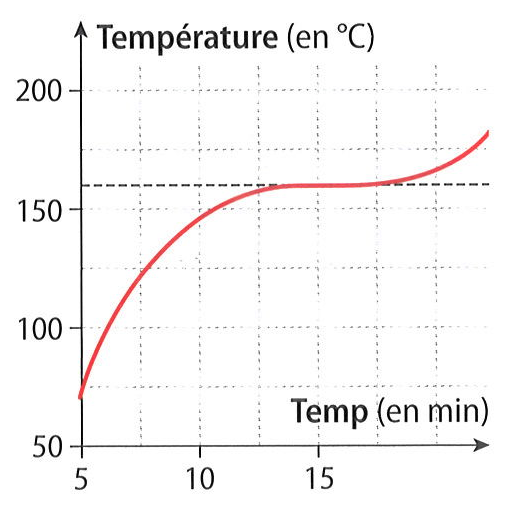
\includegraphics[scale=0.45]{./img/courbe2}
		\end{center}

		\begin{solution}
			Sur le graphique, le palier se situe entre 150°C et 175°C, ce ne peut pas être de l'ABS qui fond à une température plus importante (180°C). C'est donc du PLA qui fond à 162°C.
		\end{solution}	

>>>>>>> 30fafa87d2ff92b496b314759fcd33d498a21e3b
\end{questions}